
\chapter{Muminav}

Beispiel Progamm, welches zeigt wie man Muminav einbinden kann.

relevante andere Projekte - hoch spezifizierte Anforderungen

\section{Lizenz}

Vorgabe war, die gesamte Entwicklungsarbeit als Open Source
Projekt durchzuf�hren. Dies schlie�t ein, die
Projektergebnisse unter einer Open Source Lizenz \cite{OSI2002} zu ver�ffentlichen.\\
Da wir unser Projekt in Zusammenarbeit mit der Mumie-Gruppe
entwickeln, mussten wir uns im Vorfeld mit Ihnen auf eine Open
Source Lizenz verst�ndigen, welche in das Gesamtprojekt
\textsc{Mumie}
integrierbar ist.\\
Die GPL \cite{GPL1991} (GNU General Public License)



LGPL \cite{LGPL1999}.

\section{Entwicklungsumgebung}
\subsection{Enwicklungswerkzeuge}
F�r das Projekt wurden eine Reihe von Entwicklungswerkzeugen und
Technologien verwandt, welche f�r Open-Source-Projekte
charakteristisch sind:

\begin{itemize}

\item \textbf{Mailinglisten} um mit den Entwicklern und allen, die
sonst noch Interesse an dem Projekt haben zu kommunizieren. Wobei
damit auch gleichzeitig eine Dokumentation des Projektverlaufs
�ber die Maininglisten-Archive entsteht.
\item \textbf{CVS} Concurrent Version System \cite{FOGEL2000}.
Hat uns erm�glicht dezentral an den selben Quelldateien zu
arbeiten. �ber die CVS-Log Eintr�ge l�sst sich auch nachtr�glich
die Entwicklungs-Historie nachvollziehen.
\item \textbf{eMail} Als standard-Medium zum direkten pers�nlichen
Infromationsaustausch.
\item \textbf{Instant-Messageing} hat bei Arbeiten, die ein hohes
Ma� an Absprachen bed�rfen, nicht die Nachteile, die ein
asynchrones Medium wie eMail und Mailinglisten haben.
\item \textbf{Projekt-Homepage} Unter der URL:
\verb|http://muminav.berlios.de| haben wir eine Projekt-Homepage
angelegt, die, die �ffentlichkeit und die Teilnehmer des Projekts
mit allgemeinen Informationen versorgt.
\item \textbf{Newsgroups} Hier haben wir uns Anregungen und
Informationen f�r die Planung des Projekts und bei Problemen, die
in der t�glichen Arbeite aufraten besorgt.

%\item \textbf{}
\end{itemize}

Ant \cite{Ant2002}, JBuilder \cite{BerliOS}
\subsection{Projekthoster}

\subsection{Problemen und ihre L�sungen}

XML-Parser mitliefern - Gr��e - Entscheidung f�r Java 1.4 und
Mozilla

\section{Verwendete Komponenten und Ressourcen}

\begin{figure}[htbp]
    \centering%
%   \setcapwidth[c]{12cm}%
    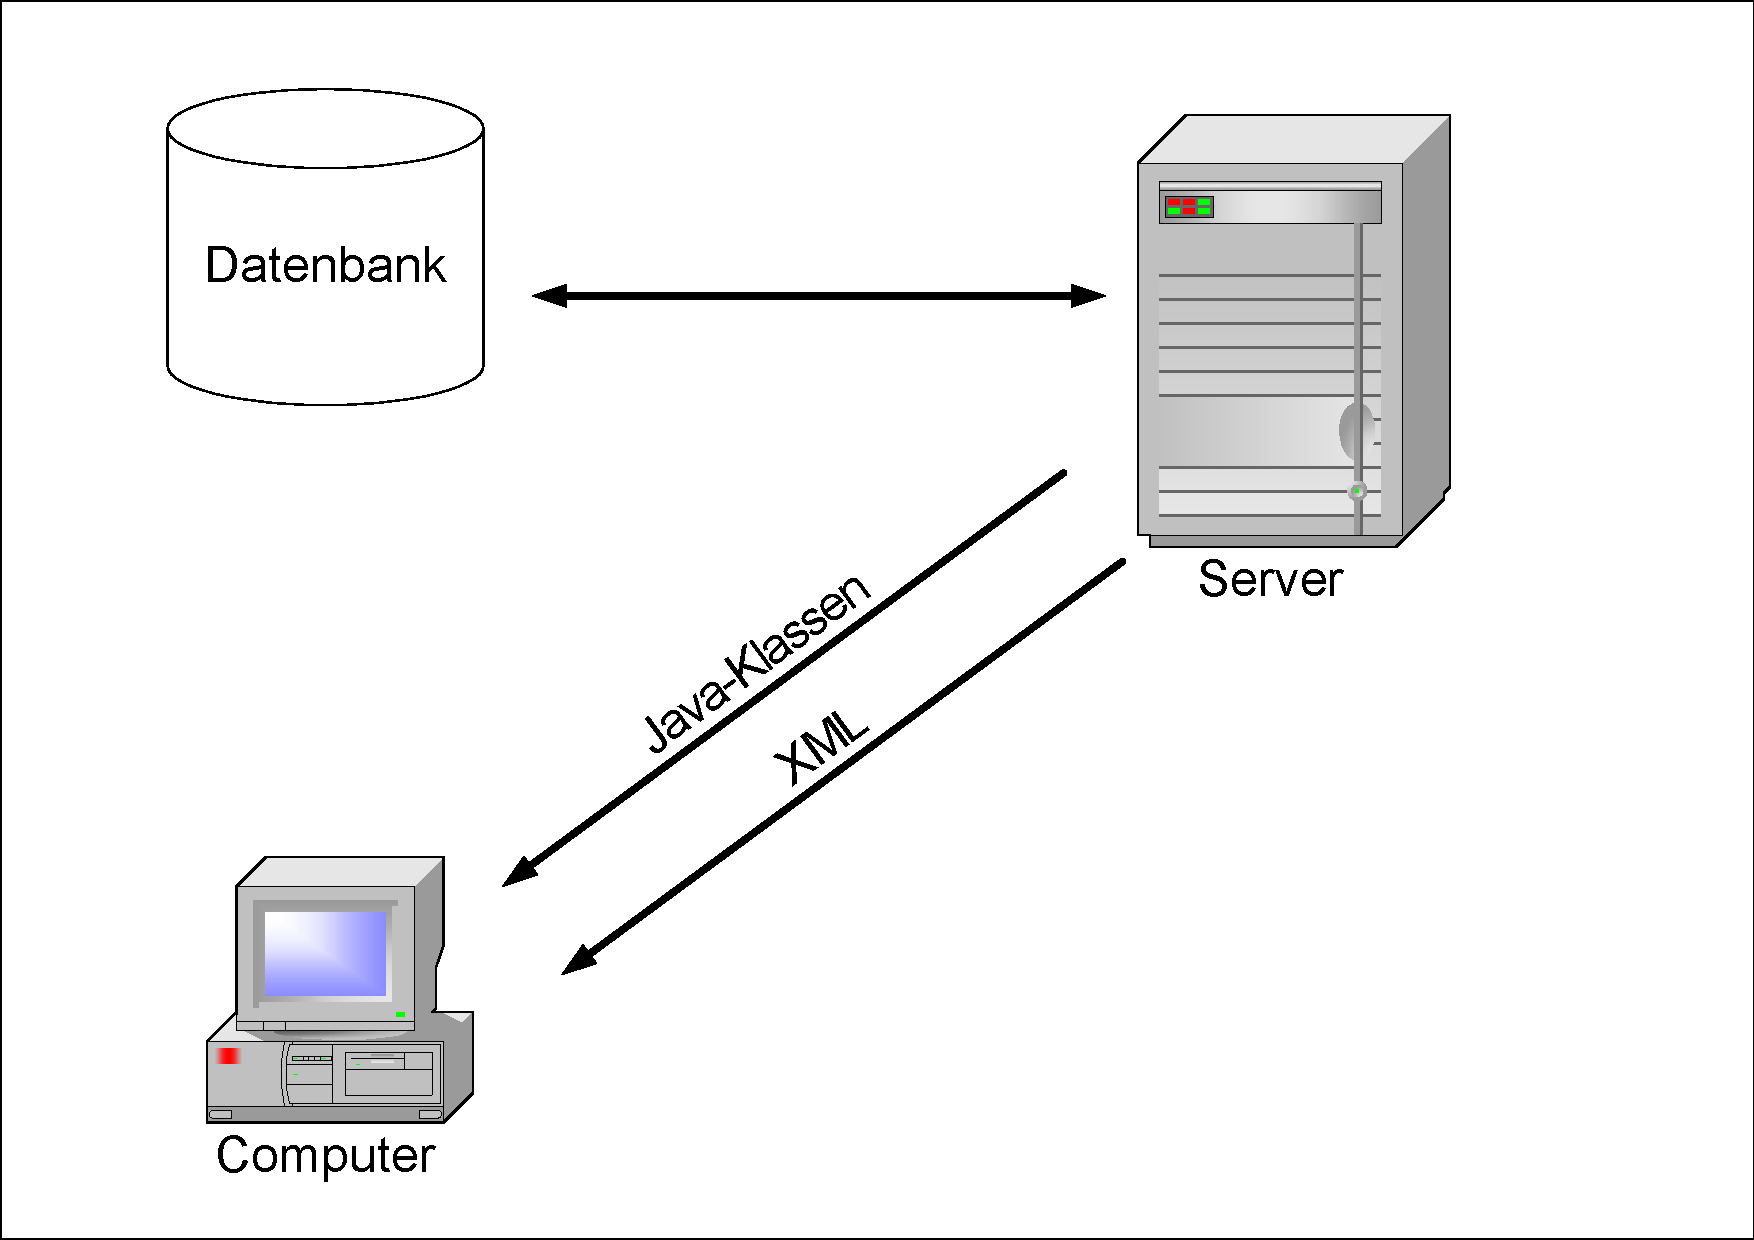
\includegraphics[width=10cm]{figs/kommunikation}
    \captionbelow{Kommunikation: Informationsfluss}
    \label{FIG:kommunikationsfluss}
\end{figure}

\begin{figure}[htbp]
    \centering%
%   \setcapwidth[c]{12cm}%
    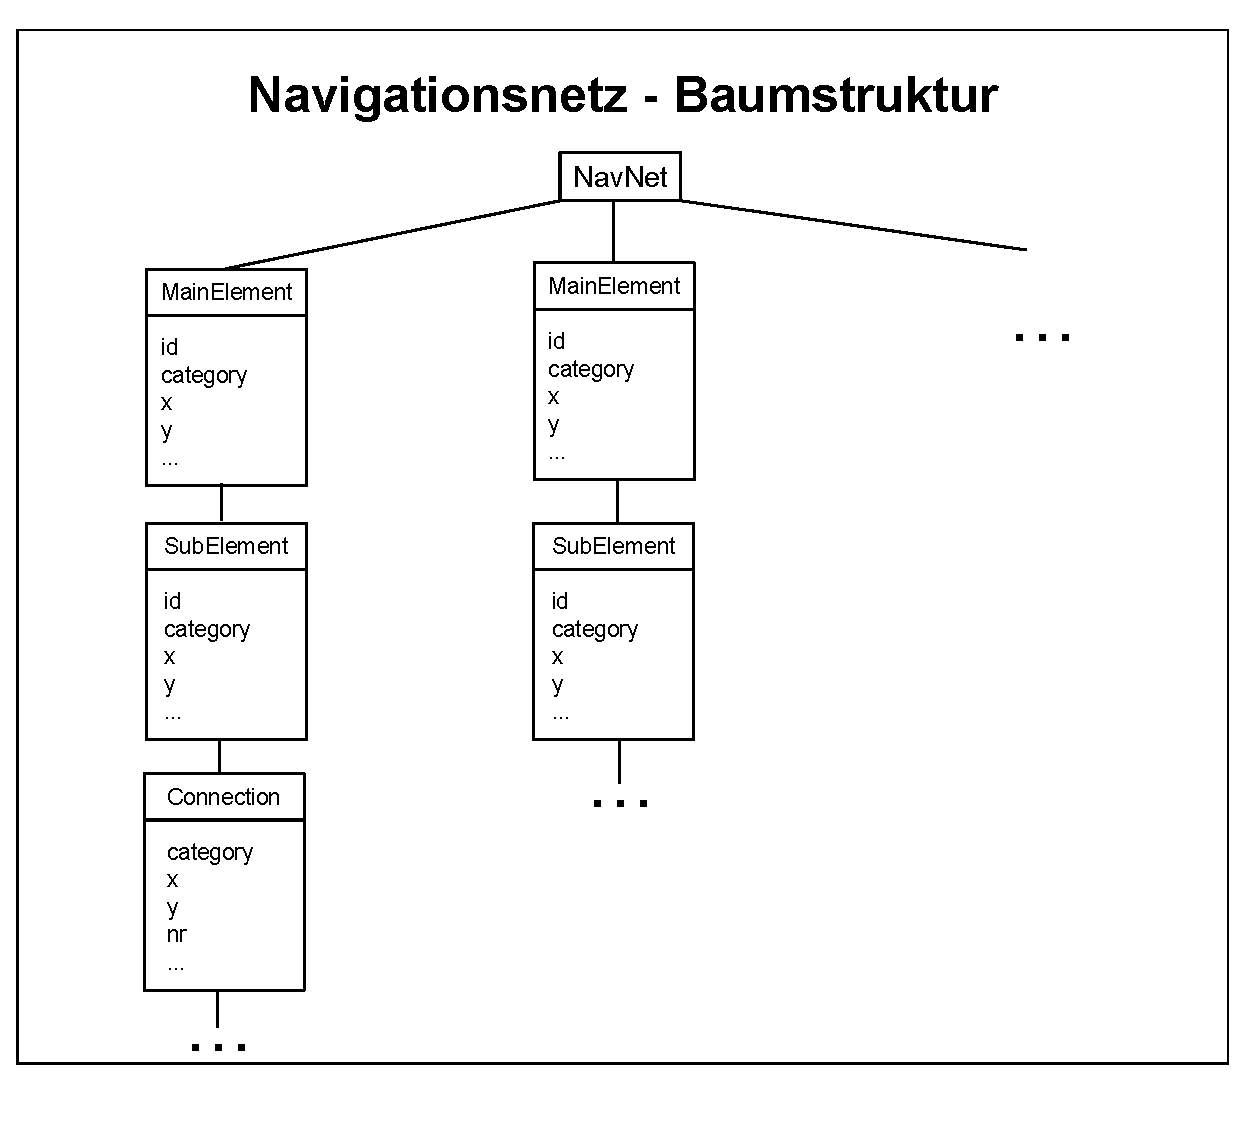
\includegraphics[width=10cm]{figs/baumstruktur}
    \captionbelow{Baumstruktur}
    \label{FIG:baumstruktur}
\end{figure}

\begin{figure}[htbp]
    \centering%
%   \setcapwidth[c]{12cm}%
    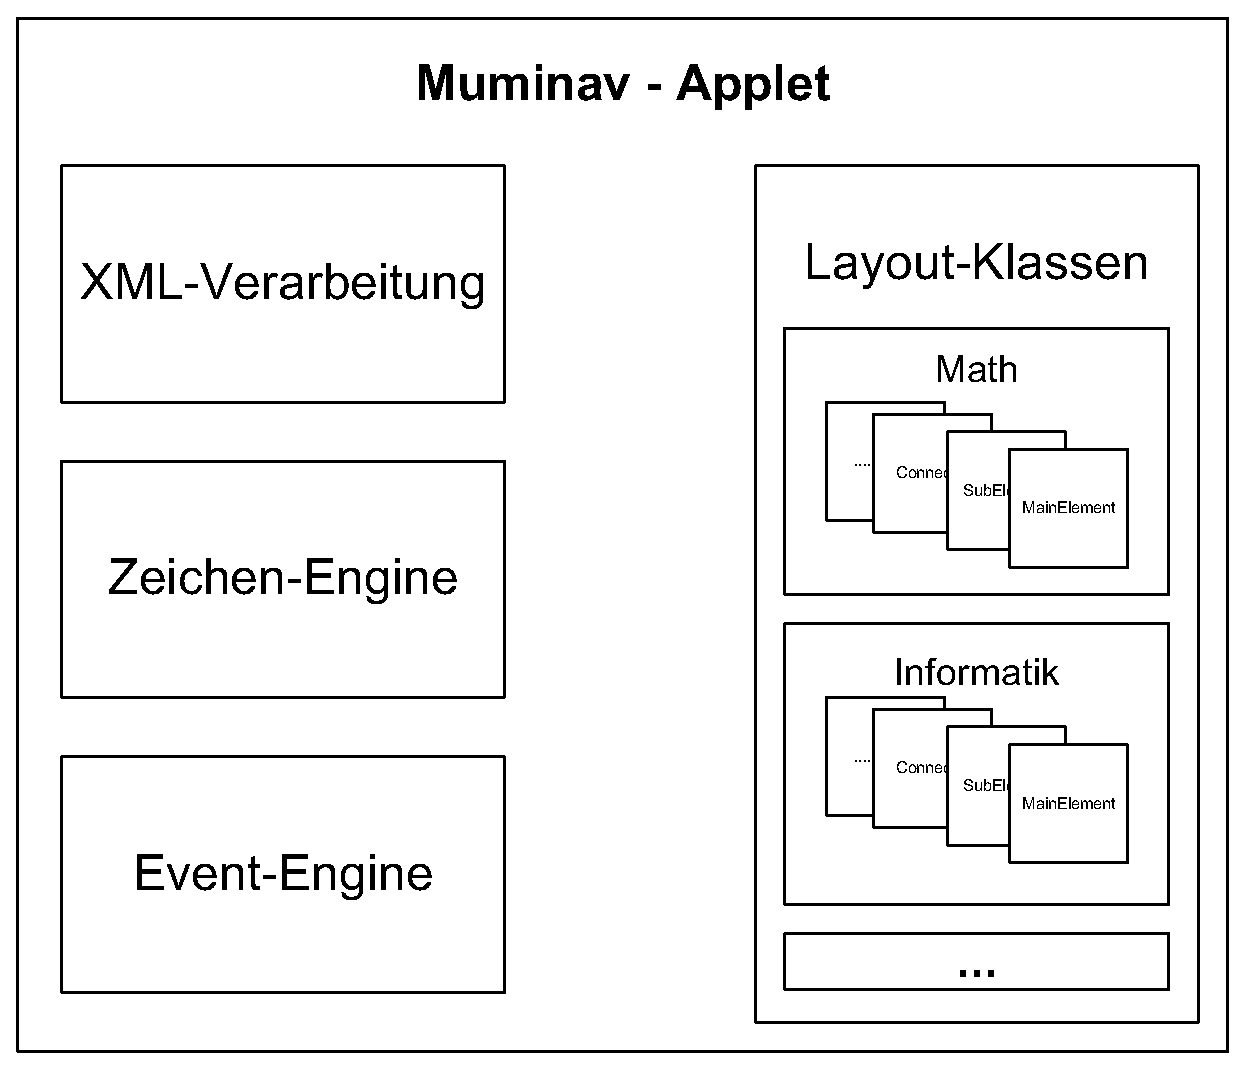
\includegraphics[width=10cm]{figs/aufbau}
    \captionbelow{Aufbau: Haupteile von Muminav}
    \label{FIG:aufbau}
\end{figure}
